\renewcommand{\theequation}{\theenumi}
\begin{enumerate}[label=\arabic*.,ref=\thesubsubsection.\theenumi]
\numberwithin{equation}{enumi}
%
\item $\vec{A} = \myvec{-2\\-2}, \vec{B} = \myvec{2\\-4}$\\
Then $\vec{P}$ that divides $\vec{A}, \vec{B}$ in the ratio k:1 is
\begin{align}
\label{section}
\vec{P} = \frac{k\vec{B}+\vec{A}}{k+1}
\end{align} 
For the given problem,$k = \frac{3}{4}$ \\
Using the equation \ref{section}, the desired point is
\begin{align}
\vec{P} = \frac{\frac{3}{4}\myvec{2\\-4}+1\myvec{-2\\-2}}{\frac{3}{4}+1} \\
\vec{P} = \myvec{-2/7\\-20/7}
\end{align}

The following python code plots the Fig.\ref{fig:line}
\begin{lstlisting}
codes/point_line/int_sec.py
\end{lstlisting}
\begin{figure}[!ht]
\centering
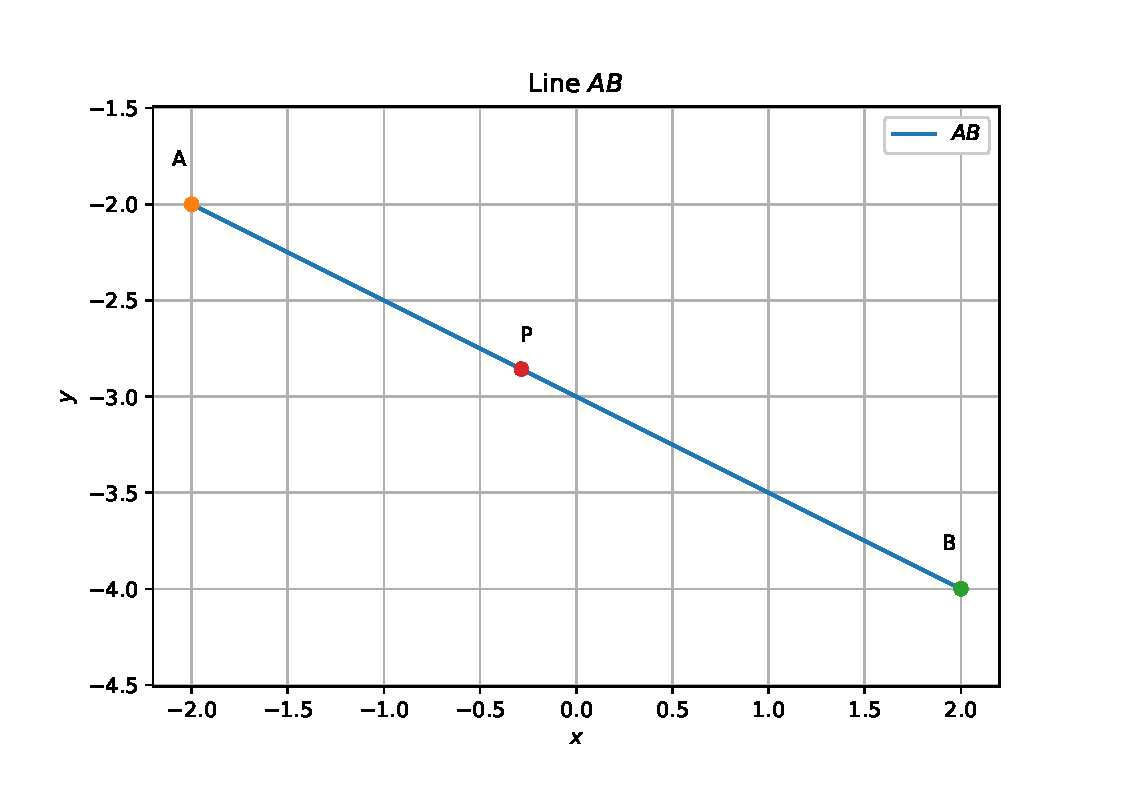
\includegraphics[width=\columnwidth]{./codes/line/point_line/int_sec.eps}
\label{fig:line}
\caption{Line $AB$ using python}
\end{figure} 

\end{enumerate}